\documentclass[tikz, margin=3.14mm]{standalone}
\usepackage{tikz}
\usetikzlibrary{positioning, arrows.meta, decorations.markings, intersections, calc, patterns, hobby, shapes.geometric, spath3, positioning}

\begin{document}
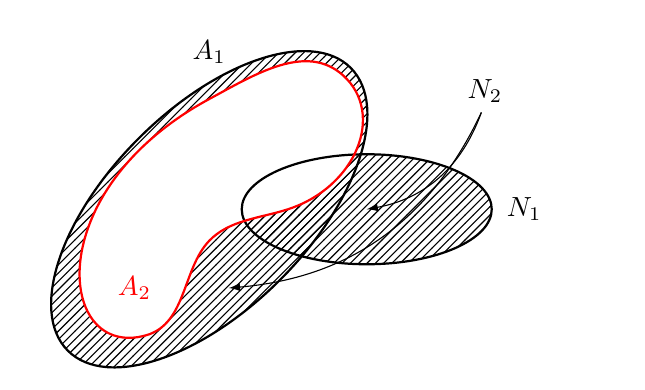
\begin{tikzpicture}[use Hobby shortcut]


% Outer curve A_1
% \draw[thick, name path=A1] ([closed]0,0)..(2.5,2)..(4,0)..(3,-4)..(0,-3)..(-1,-2)..(-1,0);





% Inner region A_2
% \draw[thick, name path=A2] (0.5,0) circle [radius=1];

% Region N_1
% \draw[thick, name path=N1] ([closed]2,2.5)..(3.5,1)..(2.5,-1)..(2,-2.5)..(0,-1.5)..(-1,-0.5)..(1,1.5);

% Region N_2
% \draw[thick, name path=N2] (0,-3)..(1,-2)..(0,-1);

% Adding slashes through (A1 \ A2) U (N1 \ A2)
\begin{scope}
    \clip [rotate=45] (0,0) ellipse (1in and .5in);% (0.5,0) circle [radius=1];
    \fill[pattern=north east lines, rotate=45, solid] (0,0) ellipse (1in and .5in);
    \fill[fill=white] ([closed]0,1.4)..(1.7,1.7)..(1,0)..(0,-.4)..(-.8,-1.6);
\end{scope}

\begin{scope}
    \clip (2,0) ellipse (1.25in and .55in);
    \fill[pattern=north east lines, solid] (2,0) ellipse (.625in and .275in);
    \fill[fill=white] ([closed]0,1.4)..(1.7,1.7)..(1,0)..(0,-.4)..(-.8,-1.6);
\end{scope}

% N1
\node[ellipse, name path = N1, thick, draw=black, minimum width=1.25in, minimum height=.55in] (N1) at (2,0) {};

% red A2
\draw[thick, draw=red, name path=A2] ([closed]0,1.4)..(1.7,1.7)..(1,0)..(0,-.4)..(-.8,-1.6);

% ellipse A 
\node[ellipse, thick, draw=black, name path = A1, rotate = 45, minimum width=2in, minimum height=1in] (A1) at (0,0) {};

\node at (0,2) {$A_1$};
\node [red] at (-.95,-1) {\color{red}$A_2$};
\node at (4, 0) {$N_1$};
\node (N2label) at (3.5, 1.5) {$N_2$};

\draw [-latex] (N2label.south west) ++(3mm,0) to [bend left] (2,0);
\draw [-latex] (N2label.south west) ++(3mm,0) to [bend left] (.25,-1);


% \begin{scope}
%     \clip (0.5,0) circle [radius=1];
%     \fill[pattern=north east lines] ([closed]2,2.5)..(3.5,1)..(2.5,-1)..(2,-2.5)..(0,-1.5)..(-1,-0.5)..(1,1.5);
%     \fill[white] (0.5,0) circle [radius=1];
% \end{scope}

% Labels
% \draw (0,0) node[above] {$A_2$};
% \draw (-2,2) node {$A_1$};
% \draw (2,2) node {$N_1$};
% \draw (0,-2.5) node {$N_2$};

\end{tikzpicture}
\end{document}
